\documentclass[tikz,border=8mm]{standalone}
\usepackage[american]{circuitikz}
\begin{document}
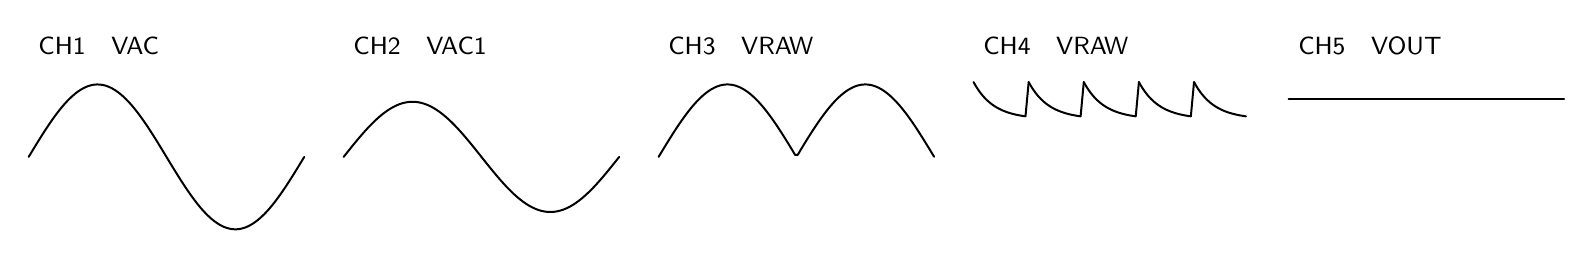
\begin{tikzpicture}[x=1cm,y=1cm,line cap=round,line join=round]
  \tikzset{
    trace/.style={draw=black,line width=.72pt}
  }

  \node[font=\sffamily\small,anchor=south west] at (0,1.18) {CH1\quad VAC};
  \node[font=\sffamily\small,anchor=south west] at (4,1.18) {CH2\quad VAC1};
  \node[font=\sffamily\small,anchor=south west] at (8,1.18) {CH3\quad VRAW};
  \node[font=\sffamily\small,anchor=south west] at (12,1.18) {CH4\quad VRAW};
  \node[font=\sffamily\small,anchor=south west] at (16,1.18) {CH5\quad VOUT};

  \draw[trace,samples=90,domain=0:3.5,smooth]
    plot (\x,{0.92*sin((\x/3.5)*360)});

  \draw[trace,samples=90,domain=4:7.5,smooth]
    plot (\x,{0.70*sin(((\x-4)/3.5)*360)});

  \draw[trace,samples=120,domain=8:11.5,smooth]
    plot (\x,{0.92*abs(sin(((\x-8)/3.5)*360))});

  % Exponential reservoir discharge and short recharge intervals.
  \foreach \a in {12,12.70,13.40,14.10,14.80}{
    \draw[trace,samples=35,domain=\a:\a+.66,smooth]
      plot (\x,{0.48+0.47*exp(-2.6*((\x-\a)/.66))});
  }
  \draw[trace] (12.66,0.52) -- (12.70,0.95)
               (13.36,0.52) -- (13.40,0.95)
               (14.06,0.52) -- (14.10,0.95)
               (14.76,0.52) -- (14.80,0.95);

  \draw[trace] (16,0.74) -- (19.5,0.74);
\end{tikzpicture}
\end{document}
